\chapter{\grapes}
\grapes (Generic Resource Aware P2P En- vironment for Streaming) is a
toolkit providing a set of \textit{generic} and \textit{reusable}
components for the development of \ptop application focused on
streaming scenarios. The fundamental philosophy behind its design is
to support as many different environment as possible while keeping at
a minimum the restrictions imposed on the applications employing it.
For these reasons it's implemented as a pure C library without any dependencies
on external libraries: as a result \grapes can be used on a variety
of systems, from high-power servers to embedded devices.

The functionality offered by the toolkit are divided into cleanly
separated modules:
\begin{itemize}
  \item \textit{Chunk Trading}, allowing to send/receive pieces of a
    media stream (called chunks);
  \item \textit{Chunk Buffer}, used to store the received chunks so
    that they can be forwarded to the other peers;
  \item \textit{Chunk ID Set} data type, that can be used to send
    signaling information about the received or needed chunks;
   \item \textit{Scheduling} functions, which can be used to decide
     which chunk to send/ask, to which peer;
   \item \textit{Network Helper}, used by the other modules and the
     applications to delegate network related tasks;
   \item \textit{Peer Set} data type, to store information about the
     nodes connected to a specific peer in the overlay (the so called
     neighbors);
   \item \textit{Peer Sampling} protocols, providing each peer with
     continuously up-to-date random samples of the entire population
     of peers.
\end{itemize}

The first four modules are not related to this work and thus will not
be covered here: for further information refer to the
\grapes paper~\cite{GRAPES}.

\ \\
The last three instead compose the fundamental blocks needed to build
the \cloudcast \peersampling protocol. The \textit{Peer Sampling} module
offers a simple implementation of \cyclon; the \textit{Peer Set}
features common set manipulation functions and support for
\textit{metadata}. In conclusion the \textit{Network Helper} greatly
simplifies the use of the network and promise the support for
\textit{NAT traversal} techniques.

In light of these facts, instead of re-implement all of the
infrastructure from scratch, it was chosen to use \grapes as a
starting point adding to it the missing components.
The rest of this chapter will cover in detail the work performed on
grapes during the course of this thesis.

\section{Groundwork}
The first issue which was identified during the initial analysis of
the toolkit was that some component (prominently the \textit{Peer
  Sampling}) were designed to support only one instance per
executable: global variables were used to maintain protocols states and
to act as buffers. Furthermore the \api did not exposed any mechanism
to select a specific instance to act on.

Such a design choice don't play well with the final aim of this work: it
would limit an application built upon it to take part in only a single
\peersampling instance. The problem was solved by \grapes authors by
having multi-process applications, where each single process is
responsible for a specific instance and communicates with other
via \emph{IPC} mechanism. Whereas this approach is both effective and
efficient when considering program written in a compiled language
such as C or C++, things rapidly changes when we shift attention to
languages requiring a \emph{virtual machine}: the aggregated memory
footprint of the application as a whole is dominated by the memory
required by the multiple \emph{VMs}. In these situations a better
approach is to keep all the application logic in a single executable
and possibly using \textit{threads} to ease the programming task.

Keeping this in mind, the first effort taken was to modify the
\emph{Peer Sampling} module to support concurrent instances. The
functions forming the high level \grapes's \api are explicitly written
to be re-entrant and should be consider thread safe, hence the only
real modification needed was the addition of execution contexts to
separate parallel instances. The task was accomplished in an
\emph{Object Oriented} inspired way: the state of each protocol was
collapsed in a C \emph{struct} which is passed as the first
argument of each \emph{Peer Sampling} \api's function thus identifying
the \emph{object} to act upon.

\ \\
Another side task which required a fairly large amount of time was the
debugging of the \emph{Peer Set}'s manipulation functions. The
first tests performed on a partial implementation of the modified
\cyclon shown odd result which greatly deviate from the simulated
behavior. After a thorough analysis a bug was found in the function
responsible for the insertion of node \descriptors in the \view.
Furthermore the \emph{Peer Set} \api was augmented with a number of
supplementary functions to manage the \textit{filling} and
\textit{sampling} of sets.

\section{Cloud Helper}
At this point the only feature \grapes missed in order to implement
\cloudcast \peersampling protocol was the support for the storage
service. A simple solution to the problem would have been to simply
relay on an external library and explicitly make use of it. Whereas
being quick and easy this strategy does not comply with the
portability requirement of the project and at the same time would have
limited the \cloud support to a single provider.

This is the rationale that lead to the introduction of the
\cloudhelper abstraction layer. This module, in line with the rest of
\grapes components, exports a simple \api (shown in
\ref{fig:grapes-cloudhelper}) which can be used by other
modules or by the final application.

\begin{figure}[H]
  \centering
  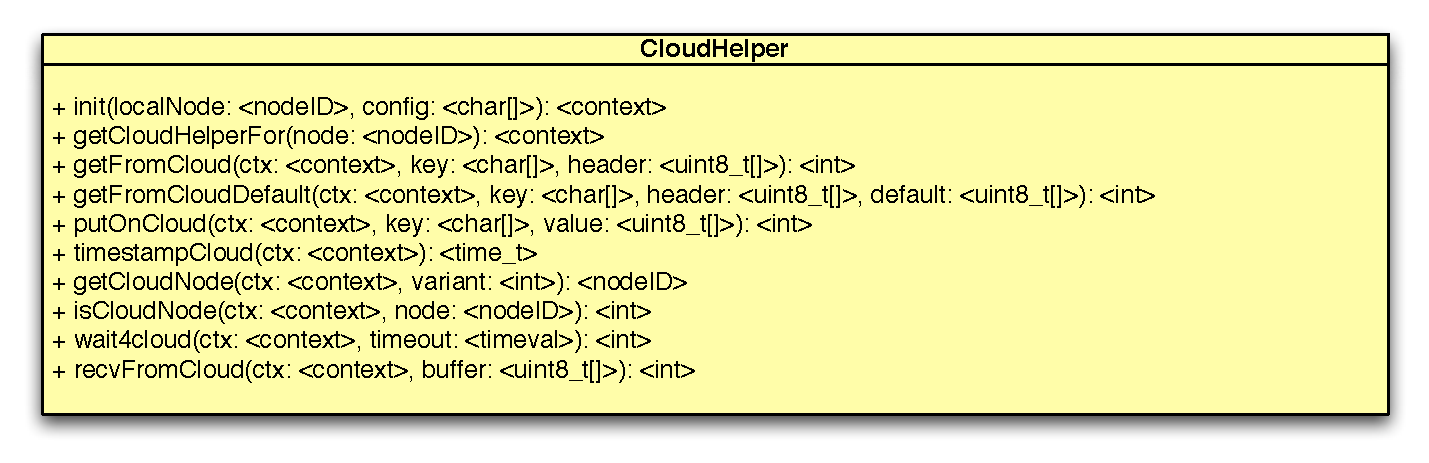
\includegraphics[width=\textwidth]{grapes-cloudhelper.pdf}
  \caption{Diagram of the \cloudhelper \api.}
  \label{fig:grapes-cloudhelper}
\end{figure}

As can be see the functionalities offered by the \api cover only the
basic \cloud operation and the support for metadata is limited to the
last modification time: indeed at the current state only those
functions needed for the \cloudcast implementation where
added.
Given that the purpose of the functions and their use is for the most
part self explanatory, in the following paragraphs it will be given
only a quick overview of them.
\emph{GetFomCloud} and \emph{getFromCloudDefault} are used to
query the \cloud for a specific \textit{key}. Both of them support the
addition of custom header to the reply to ease the processing
phase. In addition \emph{getFromCloudDefault} allows the caller to
set a default reply to be used in the event that the specified
\textit{key} is not present on the \cloud. Symmetrically
\emph{putOnCloud} takes care of updating the value of a specific
\textit{key}. These function all use plain bytes to represent
data (in the form of array of \textit{uint8\_t}) and their return
value indicates the state of the operation: $0$ is used to signal a
success while $1$ means that an error occurred while performing the
action. The \emph{timestampCloud} function is used to obtain the time
of the last modification associated to the most recent
\textit{completed} query. A query is considered \textit{completed}
when the associated response is read. This is done via the
\emph{recvFromCloud} function which stores the received data in the
specified buffer and return the number of bytes read. Application can
exploit the function \emph{wait4Cloud} to wait for the \cloud to
perform a query: a return value of $1$ indicates that the
operation was successful and the data can be read, $-1$ means that the
specified \textit{key} could not be retrieved (most likely because it's
unknown) and finally $0$ inform that some other error occurred.

The two functions \emph{getCloudNode} and \emph{isCloudNode} are used
to handle the interaction with the \textit{Peer Set} module: the
former creates new peer \descriptor using the \textit{variant}
parameter as the index of an imaginary \cloud \descriptor enumeration;
the latter instead is used to check if a specified \descriptor is
indeed referring the \cloud.

The remaining two functions are used to manage the \textit{execution
  context} of the \cloudhelper. \emph{GetCloudHelperFor} retrieve the
\textit{context} associated to a particular peer \descriptor: this
functionality is used by the \cloudcast \peersampling protocol to
fetch a configured \cloudhelper instance without requiring
modification to the current \grapes \textit{Peer Sampling} module
\api. \emph{CloudHelperInit} is the function responsible for the
creation and configuration of new \cloudhelper \textit{execution
  contexts}. Adhering to the convention in use by \grapes, this function
exploit an \textit{opaque} configuration string containing an
human readable representation of the parameters.

At the current stage the only parameter directly supported by the
\cloudhelper module is represented by the string ``\textit{provider}''
and it's used to select the actual implementation which will back the
newly created \textit{context}. Such implementation will be
responsible for parsing the remaining portion of the configuration
string.

During the course of this work two \cloudhelper implementation were
developed. The first is backed by \textit{Amazon Simple Storage
  Service} \cloud and it's based upon \textit{libS3}~\cite{LibS3}. The
second one uses a \textit{MySQL} database as storage and it
make use of \textit{MySQL Connector/C}~\cite{MySQLConnectorC}. Both
these libraries takes with them a number of dependencies and provide
synchronous operations (in contrast to the asynchronous paradigm used
by \grapes). Given the stringent restriction on dependencies and
\textit{threads} usage by the original project it was chosen not to
include the these \cloudhelper implementation directly in the code
base, instead they are available through \textit{shared libraries}.

To make this possible a \textit{fake} \cloudhelper called ``delegate''
was develop to act as a bridge between \grapes and the \textit{shared
  libraries} implementing the actual \cloud storage access. The
library name is obtained by parsing the configuration string for the parameter
``delegate\_lib''.

Figure~\ref{fig:grapes-cloudhelper-lifecycle} summarize in a schematic
fashion this process while Table~\ref{tbl:grapes-cloudhelper-libs3}
and~\ref{tbl:grapes-cloudhelper-mysql} provide a list of the provider
specific parameter they support.

\begin{figure}[H]
  \centering
  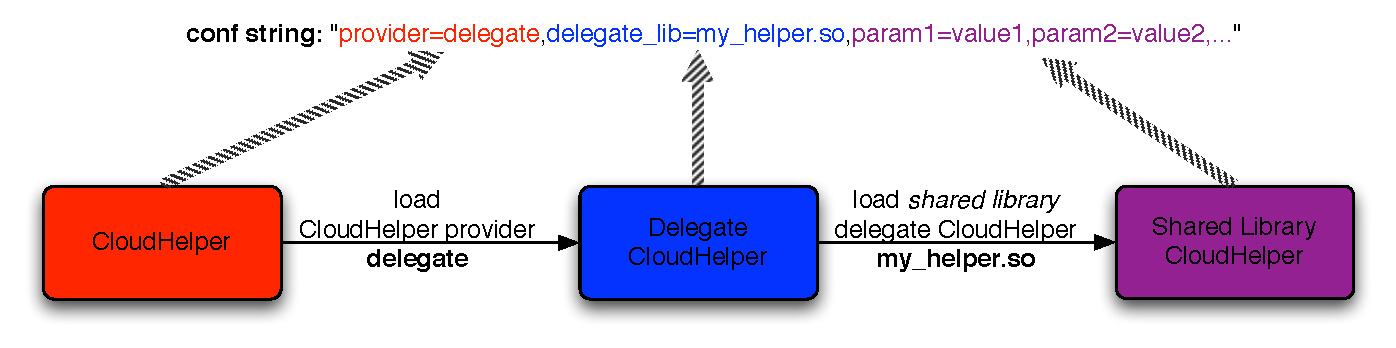
\includegraphics[width=\textwidth]{grapes-cloudhelper-lifecycle.pdf}
  \caption{\cloudhelper initialization diagram.}
  \label{fig:grapes-cloudhelper-lifecycle}
\end{figure}

\begin{table}[H]
  \centering
  \begin{tabular}{|l|l|}
  \hline
  Parameter & Meaning \\
  \hline
  \hline
  $mysql\_host$ & Hostname of the \textit{MySQL} database server \\
  $mysql\_user$ & \textit{MySQL} username \\
  $mysql\_pass$ & \textit{MySQL} password \\
  $mysql\_db$ & name of the database to use as cloud \\
  $mysql\_table$ & name of the table to use as bucket \\
  \hline
  \end{tabular}
  \caption{Provider specific parameters for \textit{MySQL} delegate helper.}
  \label{tbl:grapes-cloudhelper-mysql}
\end{table}

\begin{table}[H]
  \centering
  \begin{tabular}{|l|l|}
  \hline
  Parameter & Meaning \\
  \hline
  \hline
  $s3\_access\_key$ & \textit{Amazon} access key id \\
  $s3\_secret\_key$ & \textit{Amazon} secret access key \\
  $s3\_bucket\_name$ & name of the bucket to operate on \\
  $s3\_protocol$ & protocol used for communications. (\emph{http}  or
  \emph{https}) \\
  \hline
  \end{tabular}
  \caption{Provider specific parameters for \textit{Amazon S3} delegate helper.}
  \label{tbl:grapes-cloudhelper-libs3}
\end{table}

\section{\cloudcast \peersampling protocol}
The \cloudcast \peersampling protocol implementation is fully
integrated in the \grapes \textit{Peer Sampling} \api and doesn't
require any specific action to be taken by the final application in
order to work. The source code follows the algorithm showed in
section~\ref{sec:cloudcast-additions} and thus will not be reported
here as it does not give any substantial contribute. Instead this
section will give some insight on the configuration and usage of the
protocol.

Table \ref{tbl:grapes-cloudcast-parameters} reports the supported
configuration parameters along with their meaning and their default
value. As can be seen none of them is required to obtain a fully
functional instance, however by default the recovery mechanism
discussed in section~\ref{sec:cloudcast-additions} is not enabled
and this may cause some problem as it will be shown later on.

\begin{table}[H]
  \hspace{-20pt}
  \begin{tabular}{|p{0.27\textwidth}|p{0.63\textwidth}| c |}
  \hline
  Parameter & Meaning & Default\\
  \hline
  \hline
  $period$ & period of the active cycle (\deltacyclon) in
  seconds & 10s \\
  $cache\_size$ & size of the local \view ($c$) & 20 \\
  $sent\_entries$ & size of the partial \view ($g$) & 5\\
  $view\_key$ & key used to host the \cloud \view & ``view'' \\
  $max\_silence$ & max number of global cycle without \cloud
  contact (\maxsilence $*$ \deltacyclon) & 0 \\
  $cloud\_respawn\_prob$ & probability of creating a new \cloud
  \descriptor when silence threshold is reached (\spawnprob) defined
  in [0,1] & 0\\
  \hline
  \end{tabular}
  \caption{\cloudcast \peersampling protocol implementation
    parameters. Parenthesis enclosed values represent the
    corresponding entities in the algorithm.}
  \label{tbl:grapes-cloudcast-parameters}
\end{table}

Figure \ref{lst:grapes-example-app} shows a minimal application which
successfully takes part in a \cloudcast \peersampling protocol
instance. The differences with respect to a standard \grapes
application which exploits the \emph{Peer Sampling} module are limited
but substantial. First and most notably the \cloudhelper must be
loaded and configured, this is done in line 2 and 13-15 by including
the \textit{cloud\_helper.h} header file and by creating a new
\textit{context}. In the example the actual \cloud support is offered
by the fictional \textit{my\_helper.so} library.
The next noteworthy operation can be seen in line 16: here the actual
\peersampling protocol is loaded by specifying the value
\textit{cloudcast} for the \textit{protocol} parameter. A custom value
for the \textit{cache\_size} parameter is specified to give a better
understanding of the configuration mechanism.

The only remaining difference with respect to a standard application
regards the handling of incoming
data. Indeed given that \grapes design delegate the receiving of data
to the application, this is now responsible to read incoming messages
from both the peers and the \cloud. To help with this task, two
commodity function were developed and are exposed via the
\textit{cloud\_helper\_utils.h} header file: \textit{wait4any\_thread} and
\textit{wait4any\_polling}. The former concurrently invokes the wait
functions of the \textit{Network Helper} and \cloudhelper modules,
while the second uses a polling scheme to avoid the added dependencies
that the \textit{thread} abstraction layer takes with itself. The
first variant of this functionality can be seen in action in line 25.

These are all the information needed to successfully use the
\cloudcast \peersampling protocol implemented in \grapes in a C
application. A more exhaustive documentation of the functions discussed
in this section (and many other) is provided within the headers file
distributed alongside the source code.

\begin{figure}[H]
  \centering
  \lstinputlisting[language=C,basicstyle=\footnotesize,numberstyle=\footnotesize,numbers=left,frame=single]{code/grapes-example.c}
  \caption{Skeleton of a simple application using the \cloudcast
    \peersampling protocol.}
  \label{lst:grapes-example-app}
\end{figure}

\section{Building and deployment}
The modification to the toolkit were developed with the
support of \grapes's authors and are in the process of being merged
into the main codebase. The actual code developed during the course of
this work is available via \github~\cite{GRAPES-repo}: the tag
\thesistag point to the \emph{HEAD} revision at the moment of this
writing.

The building process is unaltered and follows the conventions
established by \grapes: to generate the main library just type ``\make''. This
will result in the creation of a \emph{static} library named
``\textit{libgrapes.a}'' containing all of the functionality apart
from the \cloudhelper delegate implementations. These must be compiled
separately by entering in the \texttt{src/CloudSupport/} directory and
typing ``\make delegate\_helpers``. Such command will generates a
separate \textit{shared} library for each available delegate
helper. The \texttt{PLATFORM} variable can be used to select the
desired library format: at the current state supported values are
\textit{unix} and \textit{darwin}.
Note that before being able to build the delegate helpers, the
\emph{libs3} and \emph{MySQL Connector/C} libraries must be
installed and configured.

\section{Java bindings}
As was mentioned in the introduction, the final goal of this work is
the creation of a general framework written in \emph{Java}. This poses
the problem of how exploit the modified \grapes toolkit from a
\emph{Java} application. In order to solve such problem a simple
library was developed to provide the bindings needed bindings. This
library is called \jgrapes.

It's designed in such a way to offer a one-to-one mapping with respect
to the \grapes's modules: the available classes are
\texttt{NetworkHelper}, \texttt{CloudHelper} and
\texttt{PeerSampler}. Each one of these exposes methods mapping the
\api of the respective \grapes module. The only design difference is
represented by the \texttt{JGrapes} class which function as a
\textit{single point of entry}: it takes care of loading the native
library and perform the required initialization action, furthermore it
provides simple function to allocate new instances of the main
components.

The usage of the library should be evident to anyone who is already
familiar with \grapes, in any case the package \emph{test} contains
a simple working application which shows the common usage.

Again the library is available via \github~\cite{jGRAPES-repo}, with
the \emph{HEAD} revision at the time of this writing tagged with
\thesistag.

The building process if fully automated and make usage of \emph{ant}
for the \emph{Java} portion and \make for the native components. The
first step is to update the \grapes distribution which will be used by
the library.
This is done by typing the command: \\
``\texttt{ant update-grapes
  -DGRAPES\_DIR=/path/to/grapes/distribution}''.

As a result both the
main \grapes library and the \cloudhelper delegate libraries will be
compiled and prepared to be used with \jgrapes. The same consideration
on the availability of the library dependencies made for
\grapes applies here so, in case of error during this phase, check
your environment.

The second step is the compilation of the \emph{Java} library
itself. This is done by invoking the target \texttt{dist} of the
\emph{ant} build file. During this second phase a series of things
happen: the final \emph{shared} library is created, the \textit{Java}
toolkit is compiled and packaged and in conclusion all the file
required to use the functionalities are placed in the \texttt{dist}
directory.
Since \jgrapes makes extensive use of \emph{JNI}~\cite{JNIGuide}, for this
phase to complete successfully, the location of \emph{JNI}'s header
files must be configured in the environment.

\section{Evaluation}
In conclusion of this chapter we would like to shows some tangible
result which shows how the real implementation perform compared with
the simulated one.
The experiments were performed via a \emph{Java} application
(available in the repository of \jgrapes) using the same configuration
parameter adopted by the corresponding simulations. When possible the
exact same setting used in the simulation was replicated, but some
specific experiment were impossible to fully reproduce due to limited
time (each simulated day requires one real day) and computational
resources.

\begin{figure}[h!]
  \centering
  \subfloat[][\emph{Cloud} in-degree]{
    \hspace{-70pt}
    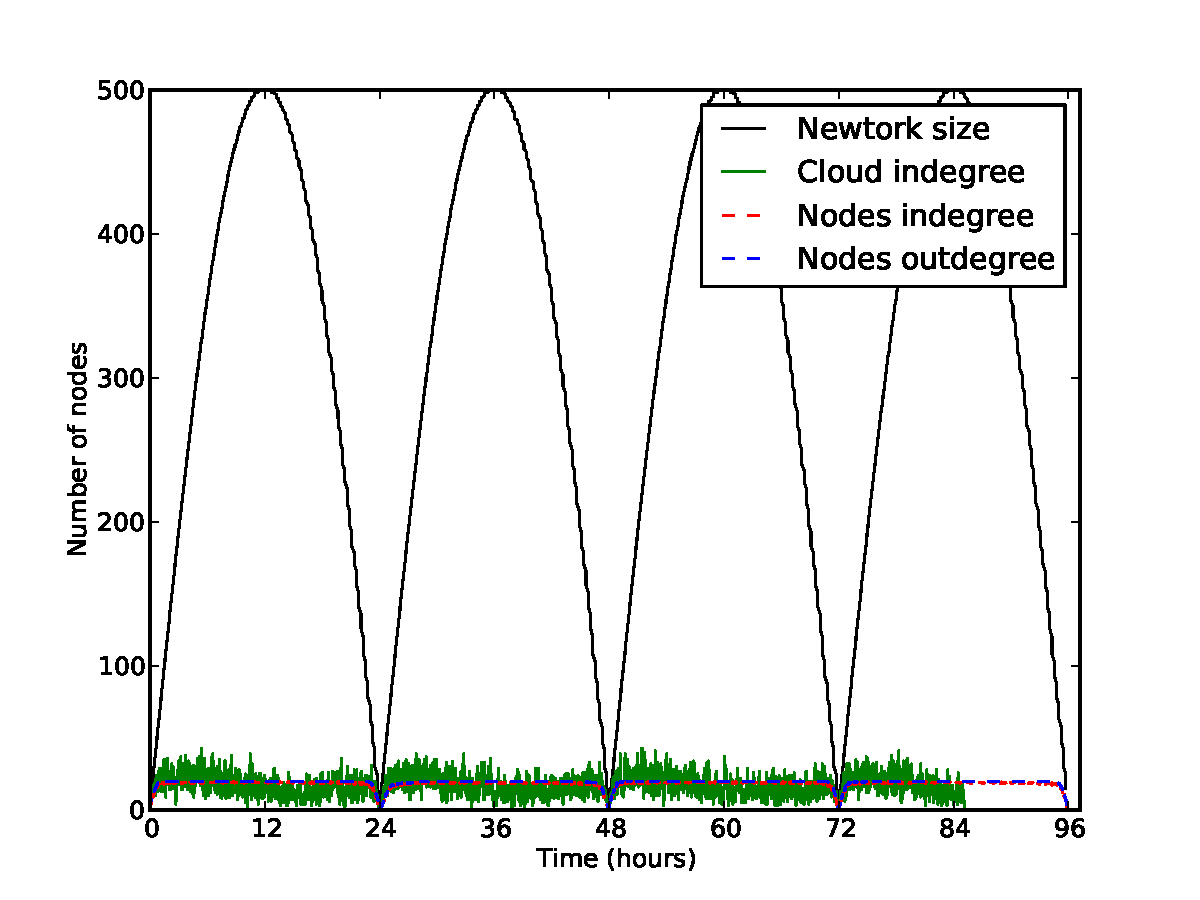
\includegraphics[width=240pt]{cloudcast-dynamic-indegree-4gg-0cloud.pdf}
    \label{fig:cloudcast-dynamic-indegree-original}
  }
  \subfloat[][\emph{Cloud} contacts]{
    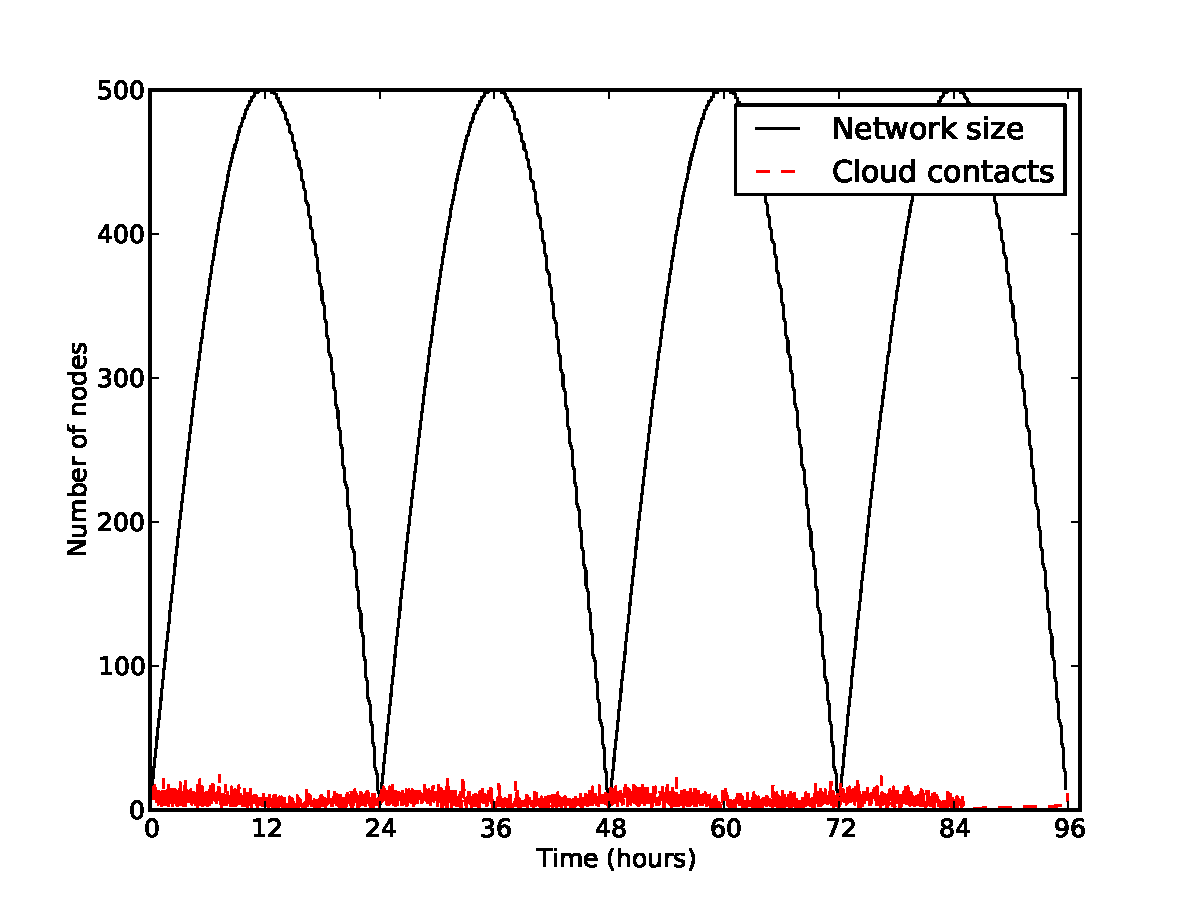
\includegraphics[width=240pt]{cloudcast-dynamic-load-4gg-0cloud.pdf}
    \label{fig:cloudcast-dynamic-load-original}
  }
  \caption{Behavior of the original \peersampling protocol}
  \label{fig:cloudcast-dynamic-original}
\end{figure}


The first result, shown in figure~\ref{fig:cloudcast-dynamic-original}
and matching figure~\ref{fig:cloudcast-sim-oscillating-indegree},
exhibit the behavior of the system when using the original protocol
without the recovery mechanism. As can be seen the protocol works as
expected for the first $3$ days, maintaining the desired \cloud
in-degree and contact rate, but as soon as the network start its
descending phase on day $4$, all the \cloud entries are lost and the
cloud is for all intent and purposes cut off the system. During the
analysis of \cloudcast it was already discussed how such a scenario
may happens, in this case however another factor plays an important
role. The way the \emph{Peer Set} module is currently implemented in
\grapes and the strategy used to maintain multiple \cloud entries by
the modified \cyclon make so that two \cloud \descriptor may be
collapsed into a single one during \view exchange. Such problem
requires a fairly extensive modification of the way \grapes handles
\descriptors to be fixed, so it wasn't feasible to fix it right
away. Anyway on its own the bug does not influences the behavior of
the protocol as it's demonstrated by the first $3$ days of execution
and by extensive tests performed on fixed size networks.

\begin{figure}[h!]
  \centering
  \subfloat[][\emph{Cloud} in-degree]{
    \hspace{-70pt}
    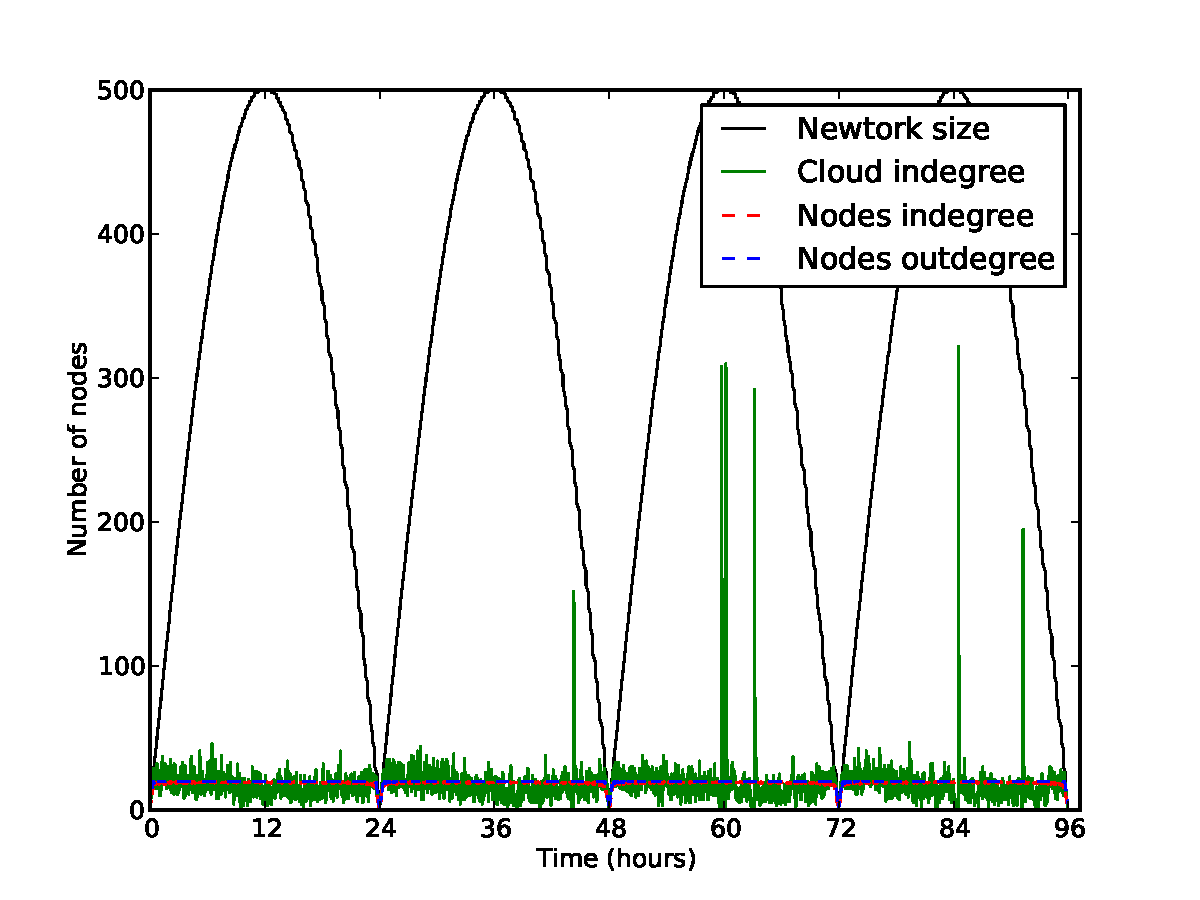
\includegraphics[width=240pt]{cloudcast-dynamic-indegree-4gg.pdf}
    \label{fig:cloudcast-dynamic-indegree-additions}
  }
  \subfloat[][\emph{Cloud} contacts]{
    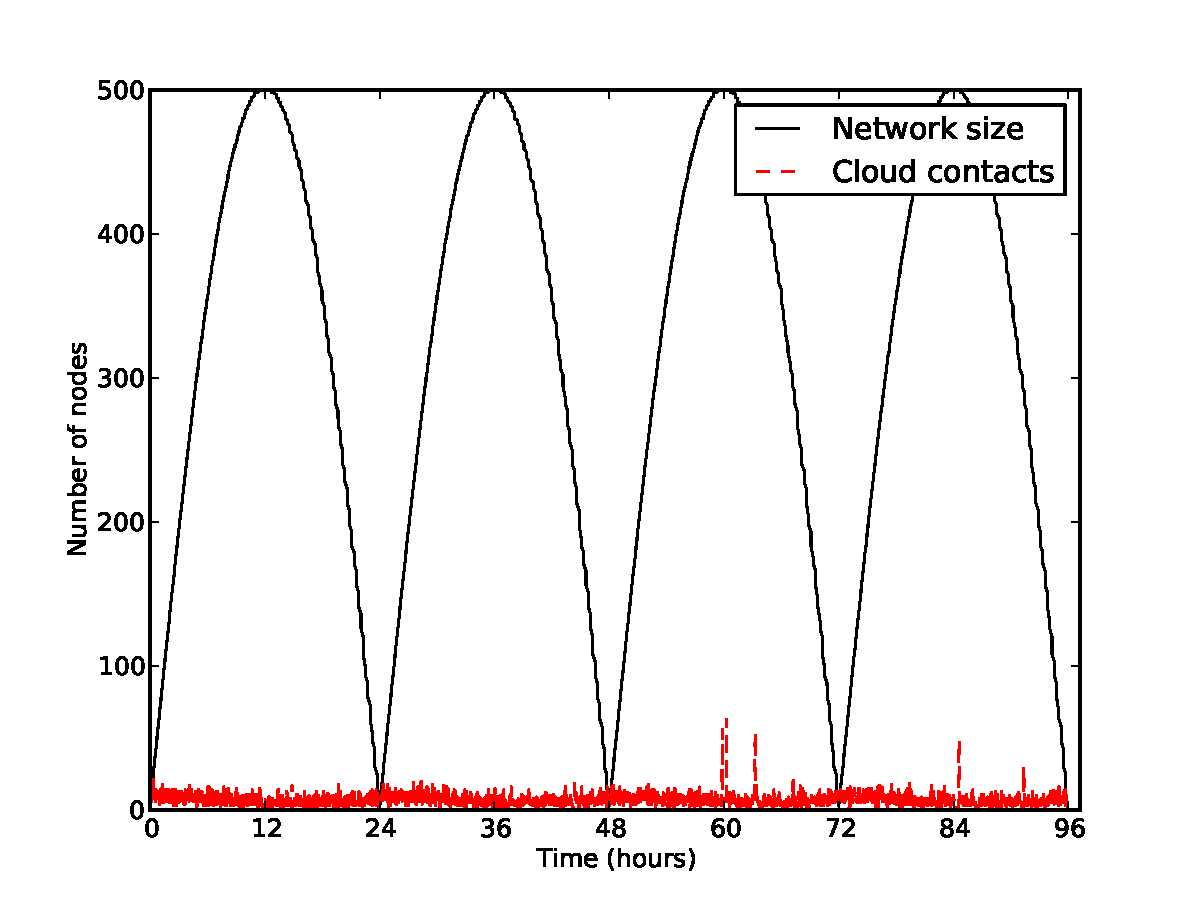
\includegraphics[width=240pt]{cloudcast-dynamic-load-4gg.pdf}
    \label{fig:cloudcast-dynamic-load-additions}
  }
  \caption{Behavior of the modified \peersampling protocol}
  \label{fig:cloudcast-dynamic-additions}
\end{figure}


Figure~\ref{fig:cloudcast-dynamic-additions} shows the same experiment
performed using the modified \cloudcast protocol. The additional
parameter used to perform these tests are:
\begin{itemize}
  \item $max\_silence$: 30 cycles
  \item $cloud\_respawn\_prob$: 0.2
\end{itemize}

The first thing that can be noted observing the
plot~\ref{fig:cloudcast-dynamic-indegree-additions} is the presence of
high peak of \cloud \descriptors. This is the effect of the recovery
mechanism in action. As can be seen the peaks are reabsorbed quickly
and as shows plot~\ref{fig:cloudcast-dynamic-load-additions} the
impact on the \cloud contact rate is fairly limited and shouldn't
impact much on the aggregated daily contacts.

\begin{figure}[h!]
  \centering
  \subfloat[][``clean'' run]{
    \hspace{-70pt}
    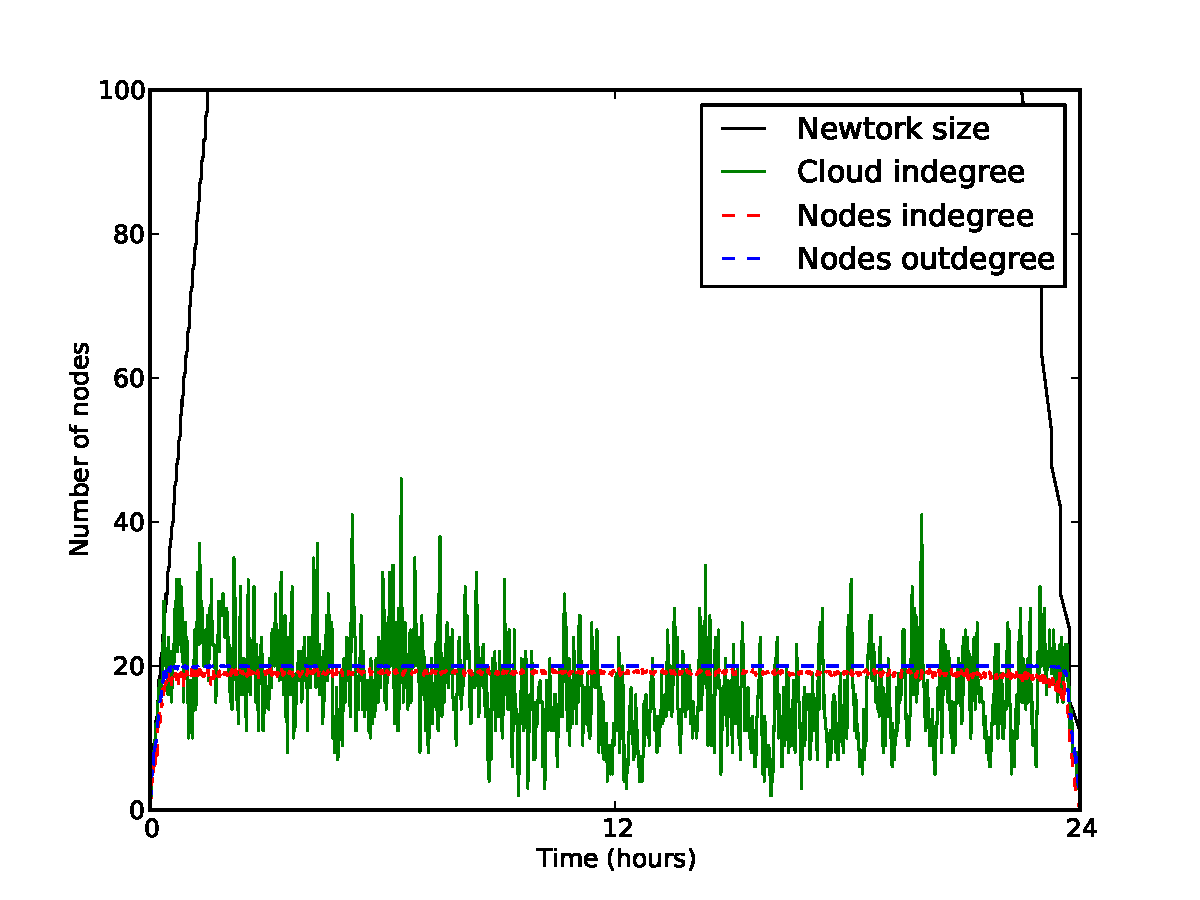
\includegraphics[width=240pt]{cloudcast-dynamic-indegree-4gg-detail-norecovery.pdf}
    \label{fig:cloudcast-dynamic-indegree-additions-detail-norecovery}
  }
  \subfloat[][Recovery mechanism in action]{
    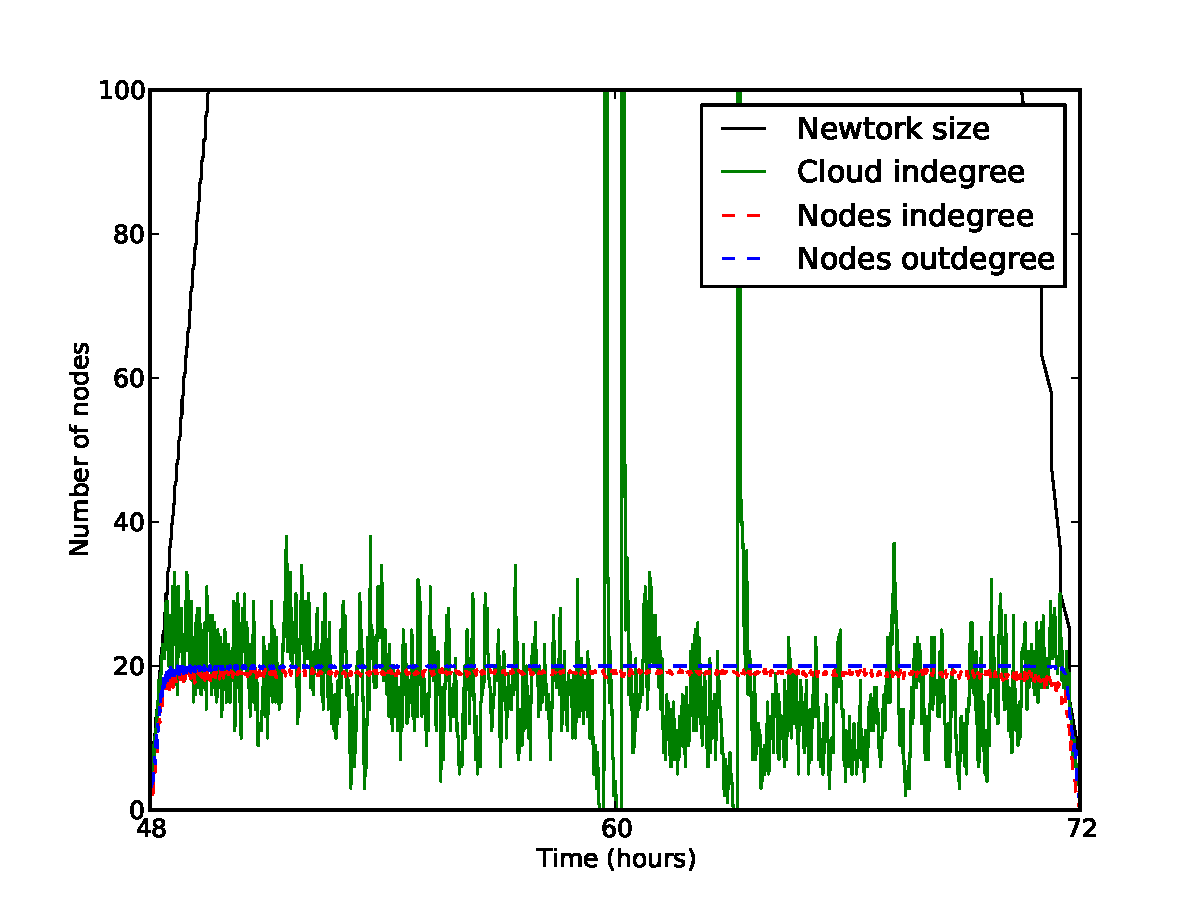
\includegraphics[width=240pt]{cloudcast-dynamic-indegree-4gg-detail-recovery.pdf}
    \label{fig:cloudcast-dynamic-indegree-additions-detail-recovery}
  }
  \caption{Zoomed in plots comparing the effects of the recovery
    mechanism on the \cloud in-degree}
  \label{fig:cloudcast-dynamic-indegree-additions-detail}
\end{figure}


Figure~\ref{fig:cloudcast-dynamic-indegree-additions-detail} shows a
comparison between ``clean'' day of execution and another in which the
recovery mechanism fired multiple times. First of all it easy to see
how the overall performance is similar in both plot: the average
number of \cloud \descriptors tend to approximate the desired value in
both plot.
More interesting is the behavior exhibited by the recovery mechanism:
around the $60^{th}$ hour of execution it is fired 2 times in a close
succession. Such a chain of events don't happen often, but it shows
how the recovery mechanism and the \cloud rate adaptive scheme works
on the two opposite fronts: the former notice that too much time is
passed since the last global \cloud contact and respond by creating a
number of \cloud \descriptors randomly distributed in the network. The
latter react to the suddenly increase in contact by removing
them.
This two competing force alongside the usual descending phase of the
network and an unlucky succession of \view exchanges have the effect
of once more removing all the \cloud entries in the network.

Considering as the starting instant the moment in which the number of
\cloud \descriptors goes to $0$ for the fist time and as ending
instant the time in which the network stabilizes itself after the
second activation of the recovery mechanism, the total time taken by
this stalling phase is around one hour. In the meantime the protocol
still works without problems even though the target \cloud contact
rate is not respected.

\begin{figure}[h!]
  \centering
  \subfloat[][``clean'' run]{
    \hspace{-70pt}
    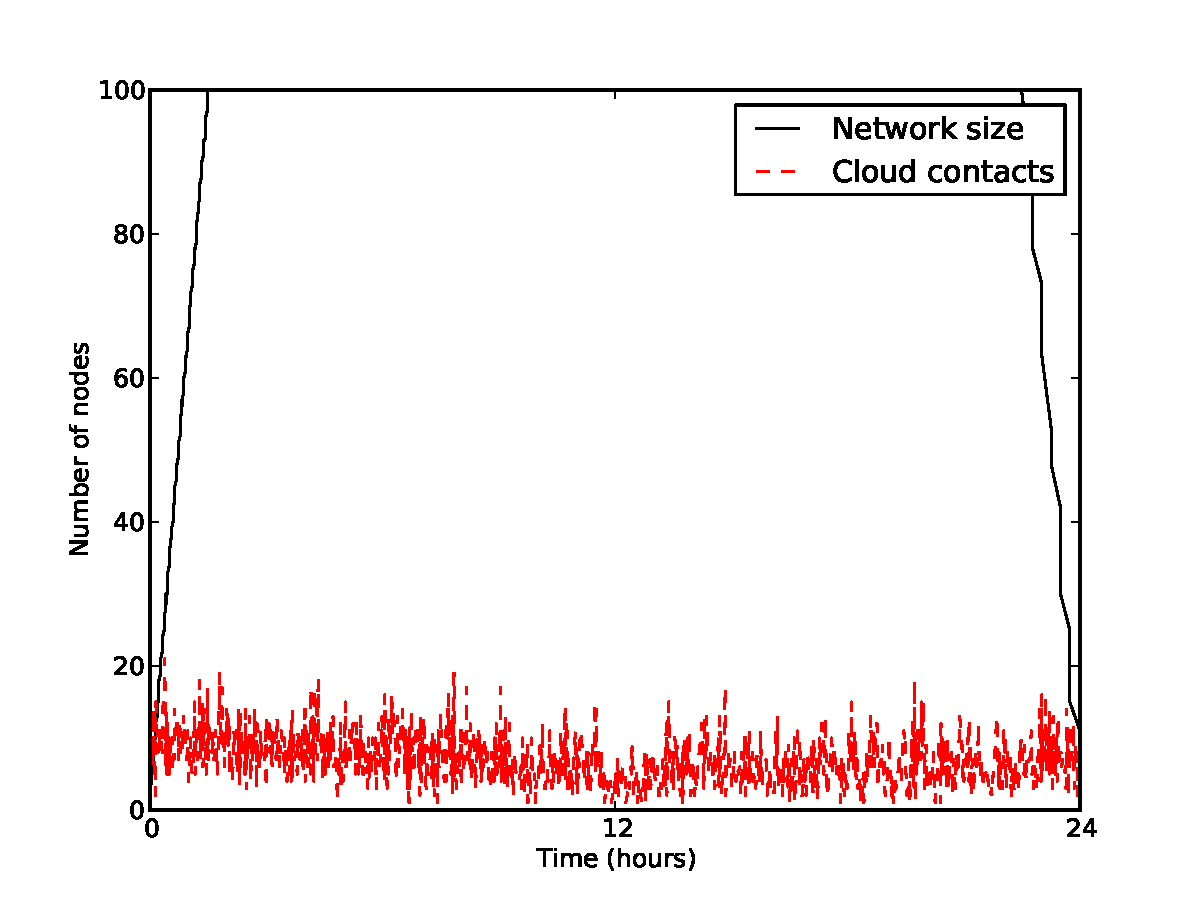
\includegraphics[width=240pt]{cloudcast-dynamic-load-4gg-detail-norecovery.pdf}
    \label{fig:cloudcast-dynamic-load-additions-detail-norecovery}
  }
  \subfloat[][Recovery mechanism in action]{
    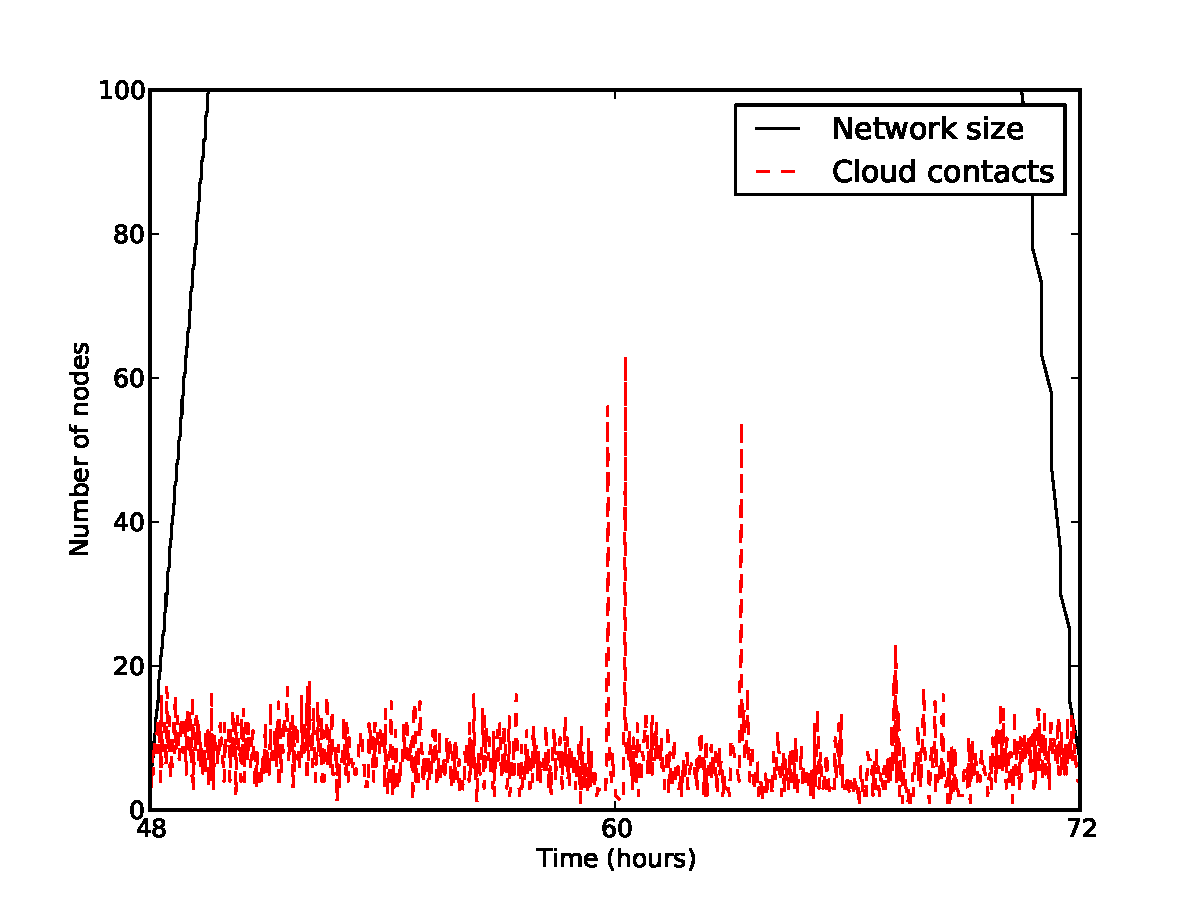
\includegraphics[width=240pt]{cloudcast-dynamic-load-4gg-detail-recovery.pdf}
    \label{fig:cloudcast-dynamic-load-additions-detail-recovery}
  }
  \caption{Detail of \cloud highlighting the effects of the recovery mechanism}
  \label{fig:cloudcast-dynamic-load-additions-detail}
\end{figure}

Figure~\ref{fig:cloudcast-dynamic-load-additions-detail} shows the
same two days from the point of view of the \cloud contact rate. In
these plot is more evident how limited is the influence of the
recovery mechanism: the peak are relatively small and they lasts for
limited amount of time.

The parameter used to configure the recovery mechanism was not
subjected to evaluation, they were selected so to be somewhat
realistic but without any deep consideration on the impact. Thus
by selecting them more carefully or even better by employing some
adaptive strategy the overall impact should sensibly decrease.

\begin{figure}[h!]
  \centering
  \subfloat[][Real implementation results]{
    \hspace{-70pt}
    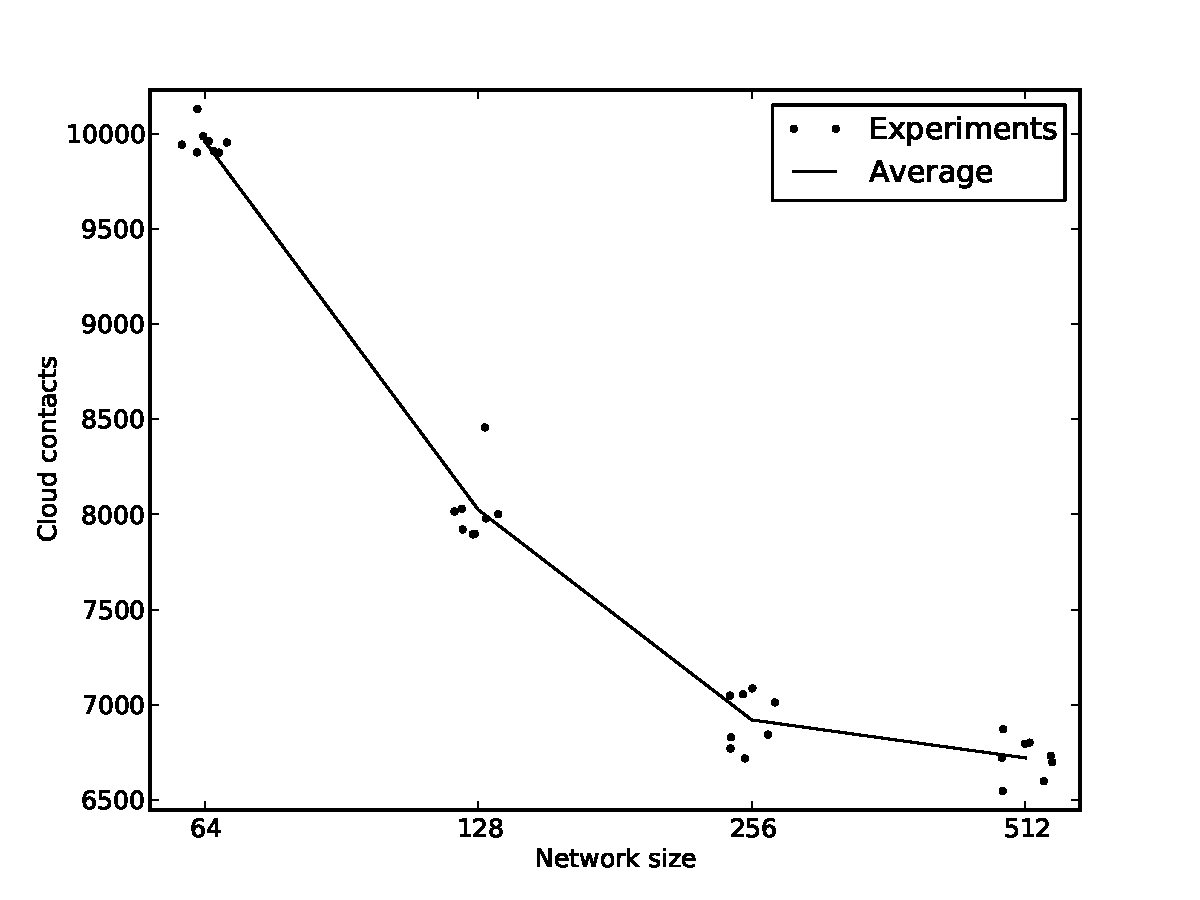
\includegraphics[width=240pt]{cloudcast-loads.pdf}
    \label{fig:cloudcast-loads}
  }
  \subfloat[][Simulated results]{
    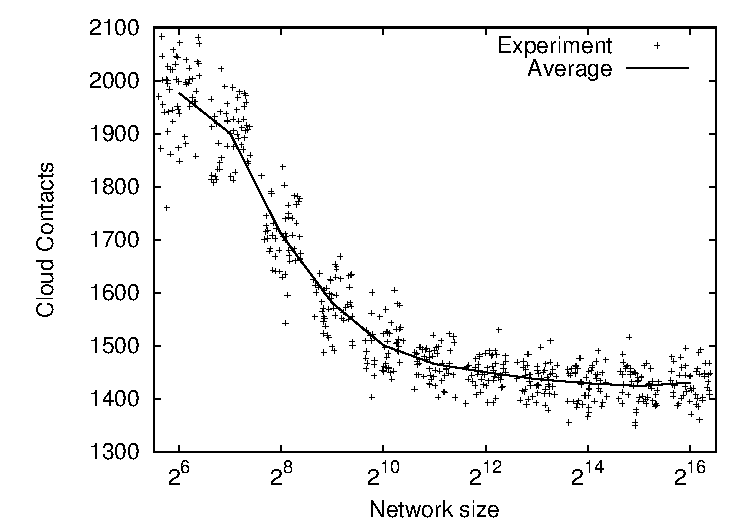
\includegraphics[width=240pt]{cloudcast-sim-loads.pdf}
    \label{fig:cloudcast-sim-loads-re}
  }
  \caption{Storage \cloud load for different network sizes.}
  \label{fig:cloudcast-loads-global}
\end{figure}

Figure~\ref{fig:cloudcast-loads-global} conclude the evaluation of the
implementations. The plot~\ref{fig:cloudcast-loads} show the \cloud
load obtained by the \grapes implementation for different network
size and match the plot in figure~\ref{fig:cloudcast-sim-loads} which
is repeated in plot~\ref{fig:cloudcast-sim-loads-re} for convenience.

Due to difference in the experiment setup and in the way data was
collected the values in the two plots are not directly comparable,
however is evident how they are proportional. In both the \cloud
contact rate is high for small networks and it tend to decrease as
more nodes are added.

The odd result obtained by the real implementation for a network size
of $1024 = 2^{10}$ is also the reason why we didn't provide samples for
denser network. The test were performed on a small number of shared
server. To simulate $1024$ nodes $4$ real machine were employed each
taking care of $256$ peers in the form of an equal number of
\emph{Java} threads. The excessive computational load posed on each
machine caused delays, missed messages and in the end resulted in the
bad performances of the protocol. Simulation with a higher number of
nodes weren't even able to run until completion.
